\section{Background}
Characters exist in the context of their past. Where did they come from? How were they raised? Backgrounds serve to enrich the characters and show how Athas shaped their story. These are ``plot complications'' to make the character feel authentic.

\subsection{Family}

\subsubsection{Family Ranking}
Athas is a harsh world, and its society reflects it in the worst ways possible---it is harshly divided into clear castes. To check your family ranking in the Athasian society, you need to roll a d10 and check your race in \tabref{Family Ranking}.

\Table{Family Ranking}{*{3}{b{6mm}b{(\columnwidth-27mm)/3}}}{
\textit{d10} & \tableheader Human, ~~~~ Half-Elf & \textit{d10} & \tableheader Dwarf & \textit{d10} & \tableheader Elf \\
1  & Noble     & 1    & Noble     & 1--2 & Merchant  \\
2  & Templar   & 2    & Templar   & 3    & Crafter   \\
3  & Merchant  & 3--4 & Merchant  & 4    & Mercenary \\
4  & Crafter   & 5--6 & Crafter   & 5--6 & Nomad     \\
5  & Mercenary & 7--8 & Mercenary & 7--8 & Raider    \\
6  & Nomad     & 9    & Hermit    & 9    & Hermit    \\
7  & Hunter    & 10   & Slave     & 10   & Slave     \\
8  & Raider    & & & & \\
9  & Hermit    & & & & \\
10 & Slave     & & & & \\

\rowcolor{white}\\
\textit{d10} & \tableheader Half-Giant & \textit{d10} & \tableheader Halfling, Thri-Kreen & \textit{d10} & \tableheader Mul \\
1     & Noble     & 1    & Crafter   & 1     & Templar   \\
2     & Templar   & 2    & Mercenary & 2     & Crafter   \\
3     & Crafter   & 3--5 & Hunter    & 3     & Mercenary \\
4--6  & Mercenary & 6--8 & Raider    & 4     & Raider    \\
7--8  & Raider    & 9    & Hermit    & 5     & Hermit    \\
9--10 & Slave     & 10   & Slave     & 6--10 & Slave     \\

\rowcolor{white}\\
\textit{d10} & \multicolumn{3}{l}{\tableheader Aarakocra, Pterran} &&\\
1--5 & Crafter   &&&& \\
6    & Mercenary &&&& \\
7--9 & Hunter    &&&& \\
10   & Hermit    &&&& \\
}

% \begin{itemize*}
% 	\item \textbf{Noble}: The nobles control the farms and the water of the cities. Usually, each noble family picks a senior member to sit on a parliamentary council.
% 	\item \textbf{Templar}: Templars are clergymen devoted to the sorcerer-king of their city. These greedy templars dominate the king's bureaucracy.
% 	\item \textbf{Merchant}: Merchants are not citizens, for the nature of their work dictates that they maintain contact with a wide variety of societies (which makes our sorcerer-kings distrustful).
% 	\item \textbf{Crafter}:  The bulk of freemen are craftsmen and artisans who keep their shops within the city walls.
% 	\item \textbf{Mercenary}: Fighting forces for hire, they make most of the bodies in the battles. From the little villages seeking protection against raiders, to the merchant houses that need to protect their precious caravans, to the city-states needing more men to fight against each other.
% 	\item \textbf{Nomad}: Nomad herdsmen live in groups called \textit{douars}. A dozen families or so that move from pasture to pasture, pausing wherever there is water and enough forage to feed their animals. When the forage is gone, they pack up their belongings and move on.
% 	\item \textbf{Hunter}: Hunting and gathering clans are small groups that make their living through hunting meat animals and foraging for edible plants.
% 	\item \textbf{Raider}: Raiders feed and clothe themselves by stealing from caravans, lonely villages, hermits, and even the cultivated fields surrounding the cities. Their tribes vary in size from a dozen individuals to several hundred, depending on the territory they work and from whom they usually steal.
% 	\item \textbf{Hermit}: Hermits come in all races and from all walks of life. They live alone in some forlorn place far away from any permanent human or demihuman society, either by their own choice or because they are outcasts.
% 	\item \textbf{Slave}: A person can become a slave in one of three ways: by being born a slave, by being captured during a war or other armed conflict, or by being sold into slavery for committing some crime or failing to pay one's debts. A member of any race or social class can become a slave, though nobles and merchants usually have friends or family who will buy their freedom for them.
% \end{itemize*}



\subsubsection{Parents}
There is a 40\% chance that something has happened to one of both parents. If so, roll a d10 and check \tabref{Something Happened to Your Parents}.

\Table{Something Happened to Your Parents}{lX}{
\textit{d10} & \tableheader Event\\
1  & Your parent(s) died in a war.\\
2  & Your parent(s) died in an accident.\\
3  & Your parent(s) were murdered.\\
4  & Your parent(s) don't remember you.\\
5  & You never knew your parent(s).\\
6  & Your parent(s) are hiding to protect you.\\
7  & You were left with relatives.\\
8  & You grew up on the streets and never had parents.\\
9  & Your parent(s) gave you to adoption.\\
10 & Your parent(s) sold you.\\
}

\begin{figure}[t!]
\centering
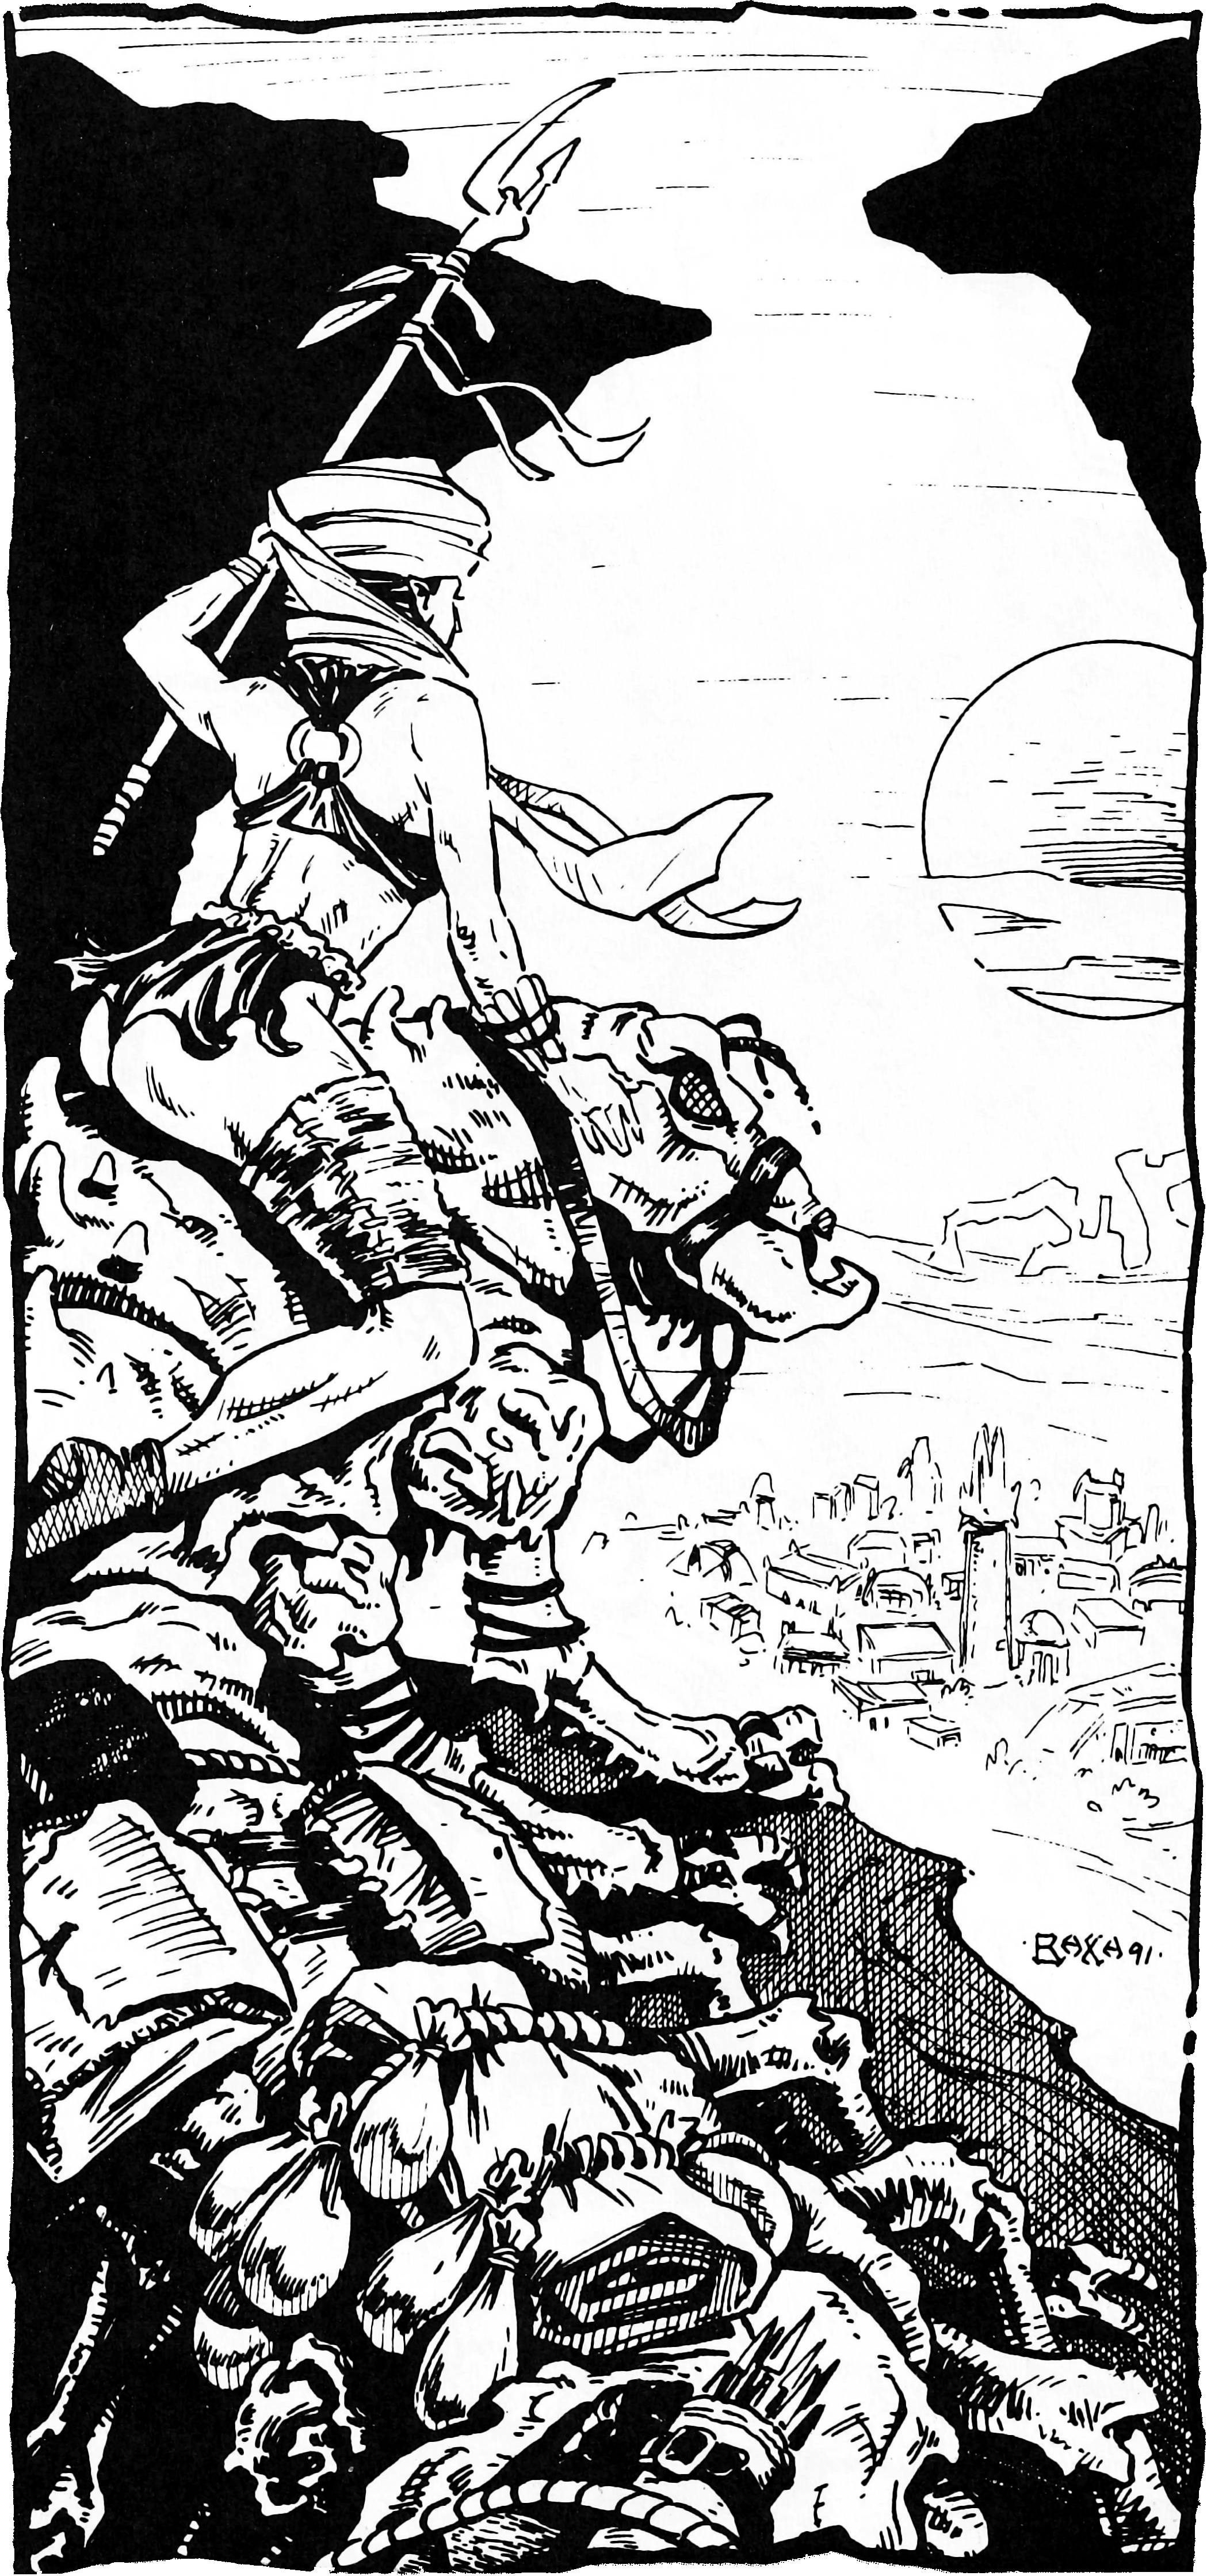
\includegraphics[width=\columnwidth]{images/ranger-1.png}
\par\textit{\small\textcopyright Wizards of the Coast, 2020.}
\end{figure}

\subsubsection{Family Status}
There is a 40\% chance that your family status is in danger. If so, roll a d10 and check \tabref{Family Tragedy}.

\Table{Family Tragedy}{lX}{
\textit{d10} & \tableheader Event\\
1  & Family lost everything through betrayal.\\
2  & Family lost everything through bad management.\\
3  & Family exiled from home.\\
4  & Family was imprisoned and you alone escaped.\\
5  & Family vanished and you are the only remaining member.\\
6  & Family was killed and you are the only survivor.\\
7  & Family is involved with the Veiled Alliance.\\
8  & Family was scattered due to misfortune.\\
9  & Family is cursed with hereditary feud.\\
10 & You are the inheritor of a family debt; you must honor this debt.\\
}

\subsubsection{Childhood}
Aarakocras and pterrans raise their children free, so there is no chance the child has an extraordinary raising. For all other races, roll 1d10 and see \tabref{Childhood Environment}.

\Table{Childhood Environment}{lX|lX}{
\textit{d10} & \multicolumn{3}{l}{\tableheader Human, Half-Elf} \\
1  & \multicolumn{3}{l}{In the Nobles' Quarter}                 \\
2  & \multicolumn{3}{l}{In a city-state}                        \\
3  & \multicolumn{3}{l}{In merchant's outpost}                  \\
4  & \multicolumn{3}{l}{Spent on the streets}                   \\
5  & \multicolumn{3}{l}{In decaying village}   \\
6  & \multicolumn{3}{l}{In a douar}                             \\
7  & \multicolumn{3}{l}{In a hunter-gatherer clan}              \\
8  & \multicolumn{3}{l}{In a raiders tribe}                     \\
9  & \multicolumn{3}{l}{In a pirate pack in the Sea of Salt}    \\
10 & \multicolumn{3}{l}{In slavery}                             \\

\rowcolor{white}\\
\textit{d10} & \tableheader Dwarf            & \textit{d10} & \tableheader Elf \\
1     & In the Nobles' Quarter               & 1    & In a city-state          \\
2--3  & In a city-state                      & 2--3 & In merchant's outpost    \\
4--5  & In merchant's outpost                & 4    & Spent on the streets     \\
6     & Spent on the streets                 & 5--6 & In a douar               \\
7--8  & In decaying village & 7--8 & In a raiders tribe       \\
9--10 & In slavery                           & 10   & In slavery               \\

\rowcolor{white}\\
\textit{d10} & \tableheader Half-Giant & \textit{d10} & \tableheader Mul              \\
1    & In the Nobles' Quarter          & 1     & In a city-state                      \\
2--4 & In a city-state                 & 2     & In merchant's outpost                \\
5    & In merchant's outpost           & 3     & Spent on the streets                 \\
6--7 & Spent on the streets            & 4     & In decaying village \\
8--9 & In a raiders tribe              & 5     & In a raiders tribe                   \\
10   & In slavery                      & 6--10 & In slavery                           \\

\rowcolor{white}\\
\textit{d10} & \multicolumn{3}{l}{\tableheader Halfling, Thri-kreen} \\
1--2 & \multicolumn{3}{l}{In decaying village}      \\
4--6 & \multicolumn{3}{l}{In a hunter-gatherer clan}                 \\
7--9 & \multicolumn{3}{l}{In a raiders tribe}                        \\
10   & \multicolumn{3}{l}{In slavery}                                \\
}

\begin{figure}[t!]
\centering
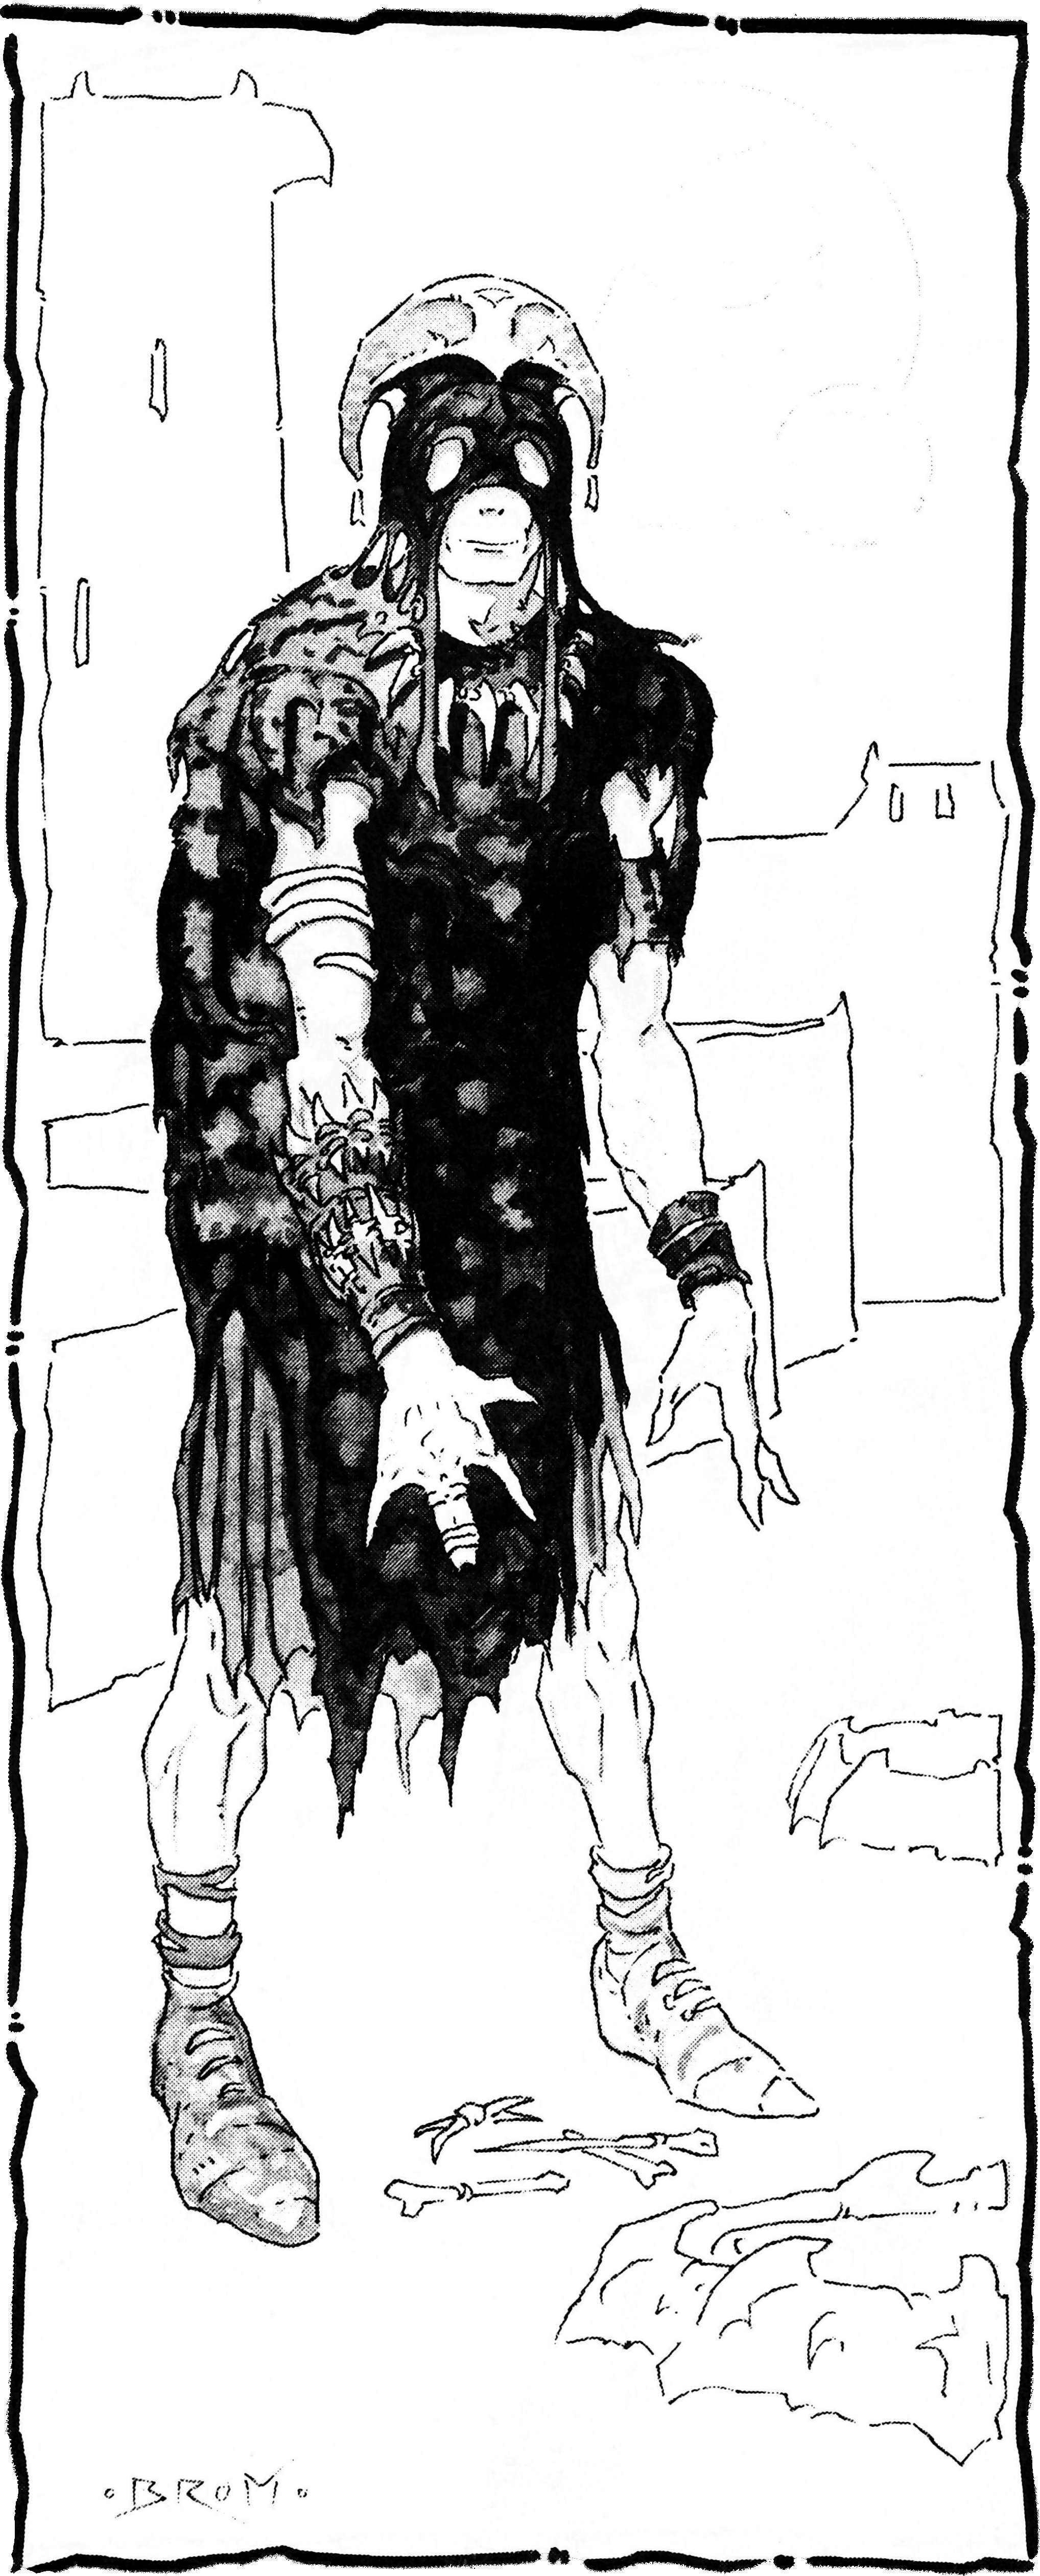
\includegraphics[width=\columnwidth]{images/wiz-1.png}
\par\textit{\small\textcopyright Wizards of the Coast, 2020.}
\end{figure}

\subsubsection{Siblings}
Determine the number of siblings you have by rolling your race's dice (see below). You are an only child if you roll a result within your race's margin.

\Table{}{Xcc}{
\tableheader Race & \tableheader Die & \tableheader Only Child Margin\\
Aarakocra, half-giant, pterran & 1d6 & 5--6\\
Dwarf & 1d12 & 10--12 \\
Elf, human, half-elf, halfling, mul & 1d10 & 8--10\\
Thri-kreen & 1d20 & 18--20\\
}

For each sibling roll a die. If the result is even, the sibling is male, else the sibling is female. Then roll for each step in \tabref{Sibling}.

\Table{Sibling}{lX}{
\textit{d10} & \tableheader Relative age\\
1--5 & Sibling is older.\\
6--9 & Sibling is younger.\\
10 & Sibling is your twin.\\

\cmidrule[0pt]{1-2}
\rowcolor{white}\\
\textit{d10} & \tableheader Feelings towards you\\
1--2  & Sibling dislikes you.\\
3--4  & Sibling likes you.\\
5--6  & Sibling is neutral towards you.\\
7--8  & Sibling hero worship you.\\
9--10 & Sibling hates you.\\ 
}

\subsection{Life Events}
For each year of your character's life past your race's adulthood age (see \tabref{Random Starting Ages}), roll 1d6 to see the next step:

\Table{Life Events}{lX}{
\textit{d6} & \tableheader Next Step \\
1--2 & Big event \\
3--4 & Friends \& Enemies \\
5 & Romance \\
6 & Nothing happened\\
}

\subsubsection{Big Event}
Roll a die. On an even roll, you got lucky---roll 1d10 and check \tabref{Lucky Event}. On an odd roll, something bad happened---roll 1d10 and check \tabref{Disaster Event}.

\Table{Lucky Event}{lX}{
\textit{d10} & \tableheader Event \\
1  & \textbf{Make a Powerful Connection}: Roll 1d6. 1--2: it's in the templarate. 3--4: it's in a large merchant house. 5--6: it's in the Veiled Alliance.\\
2  & \textbf{Financial Windfall}: Gain 1d4 $\times$ 10 cp.\\
3  & \textbf{Financial Windfall}: Gain 1d4 $\times$ 10 cp.\\
4  & \textbf{Find a Sensei}: Gain 1 power point.\\
5  & \textbf{Find a Teacher}: Gain 1 skill point.\\
6  & \textbf{Powerful Merchant} owes you one favor.\\
7  & \textbf{Local raider tribe befriends you}. You can call them for 1 favor/month.\\
8  & \textbf{Make a friend on the Templarate}. You gain +2 in \skill{Gather Information} in a city-state.\\
9  & \textbf{Local wizards like you}. You can call them for 1 favor/month.\\
10 & \textbf{Find a Combat Teacher}: You gain \feat{Weapon Focus} on a simple weapon.\\
}

\Table{Disaster Event}{lX}{
\textit{d10} & \tableheader Event \\
1 & \textbf{Debt}: You lose 1d4 $\times$ 10 cp. If you can't pay this now, you have a debt to pay, in cash---or blood.\\
2 & \textbf{Imprisonment}: You were in prison or held hostage for 1d12 months.\\
3 & \textbf{Illness or addiction}: You have contracted either an illness or drug habit in this time.\\
4 & \textbf{Betrayal}: Roll 1d6. 1--2: you are being blackmailed. 3--4: a secret was exposed. 5--6: you were betrayed by a close friend.\\
5 & \textbf{Accident}: Roll 1d4. 1--2: you were disfigured and gain --5 in \skill{Diplomacy}. 3: you have lost 1d12 months of memory of that year. 4: you constantly relive nightmares of the accident and wake up screaming.\\
6 & \textbf{Lover, friend or relative killed}: Roll 1d6. 1--3: they died accidentally. 4--5: they were murdered by unknown parties. 6: they were murdered and you know who did it.\\
7 & \textbf{False Accusation}: Roll 1d10. 1--3: it's theft. 4--5: it's wizardry. 6--8: it's murder. 9: it's rape. 10: it's lying or betrayal.\\
8 & \textbf{Hunted by the Law}: Roll 1d6. 1--2: only local guards want you. 3--4: it's the entire city's guard. 5: it's the templarate. 6: all templarates are after you.\\
9 & \textbf{Hunted by a Merchant House}: Roll 1d6. 1--2: it's only a local shop. 3--4: it's a small merchant house. 5: it's a large merchant house. 6: all major houses are after you.\\
10& \textbf{Mental or physical incapacitation}: Roll 1d6. 1--2: a nervous disorder, $-1$ in Fort. 3--4: a mental problem, $-1$ in Will. 5--6: a major psychosis, $-1$ Ref.\\
}

\begin{figure}[t!]
\centering
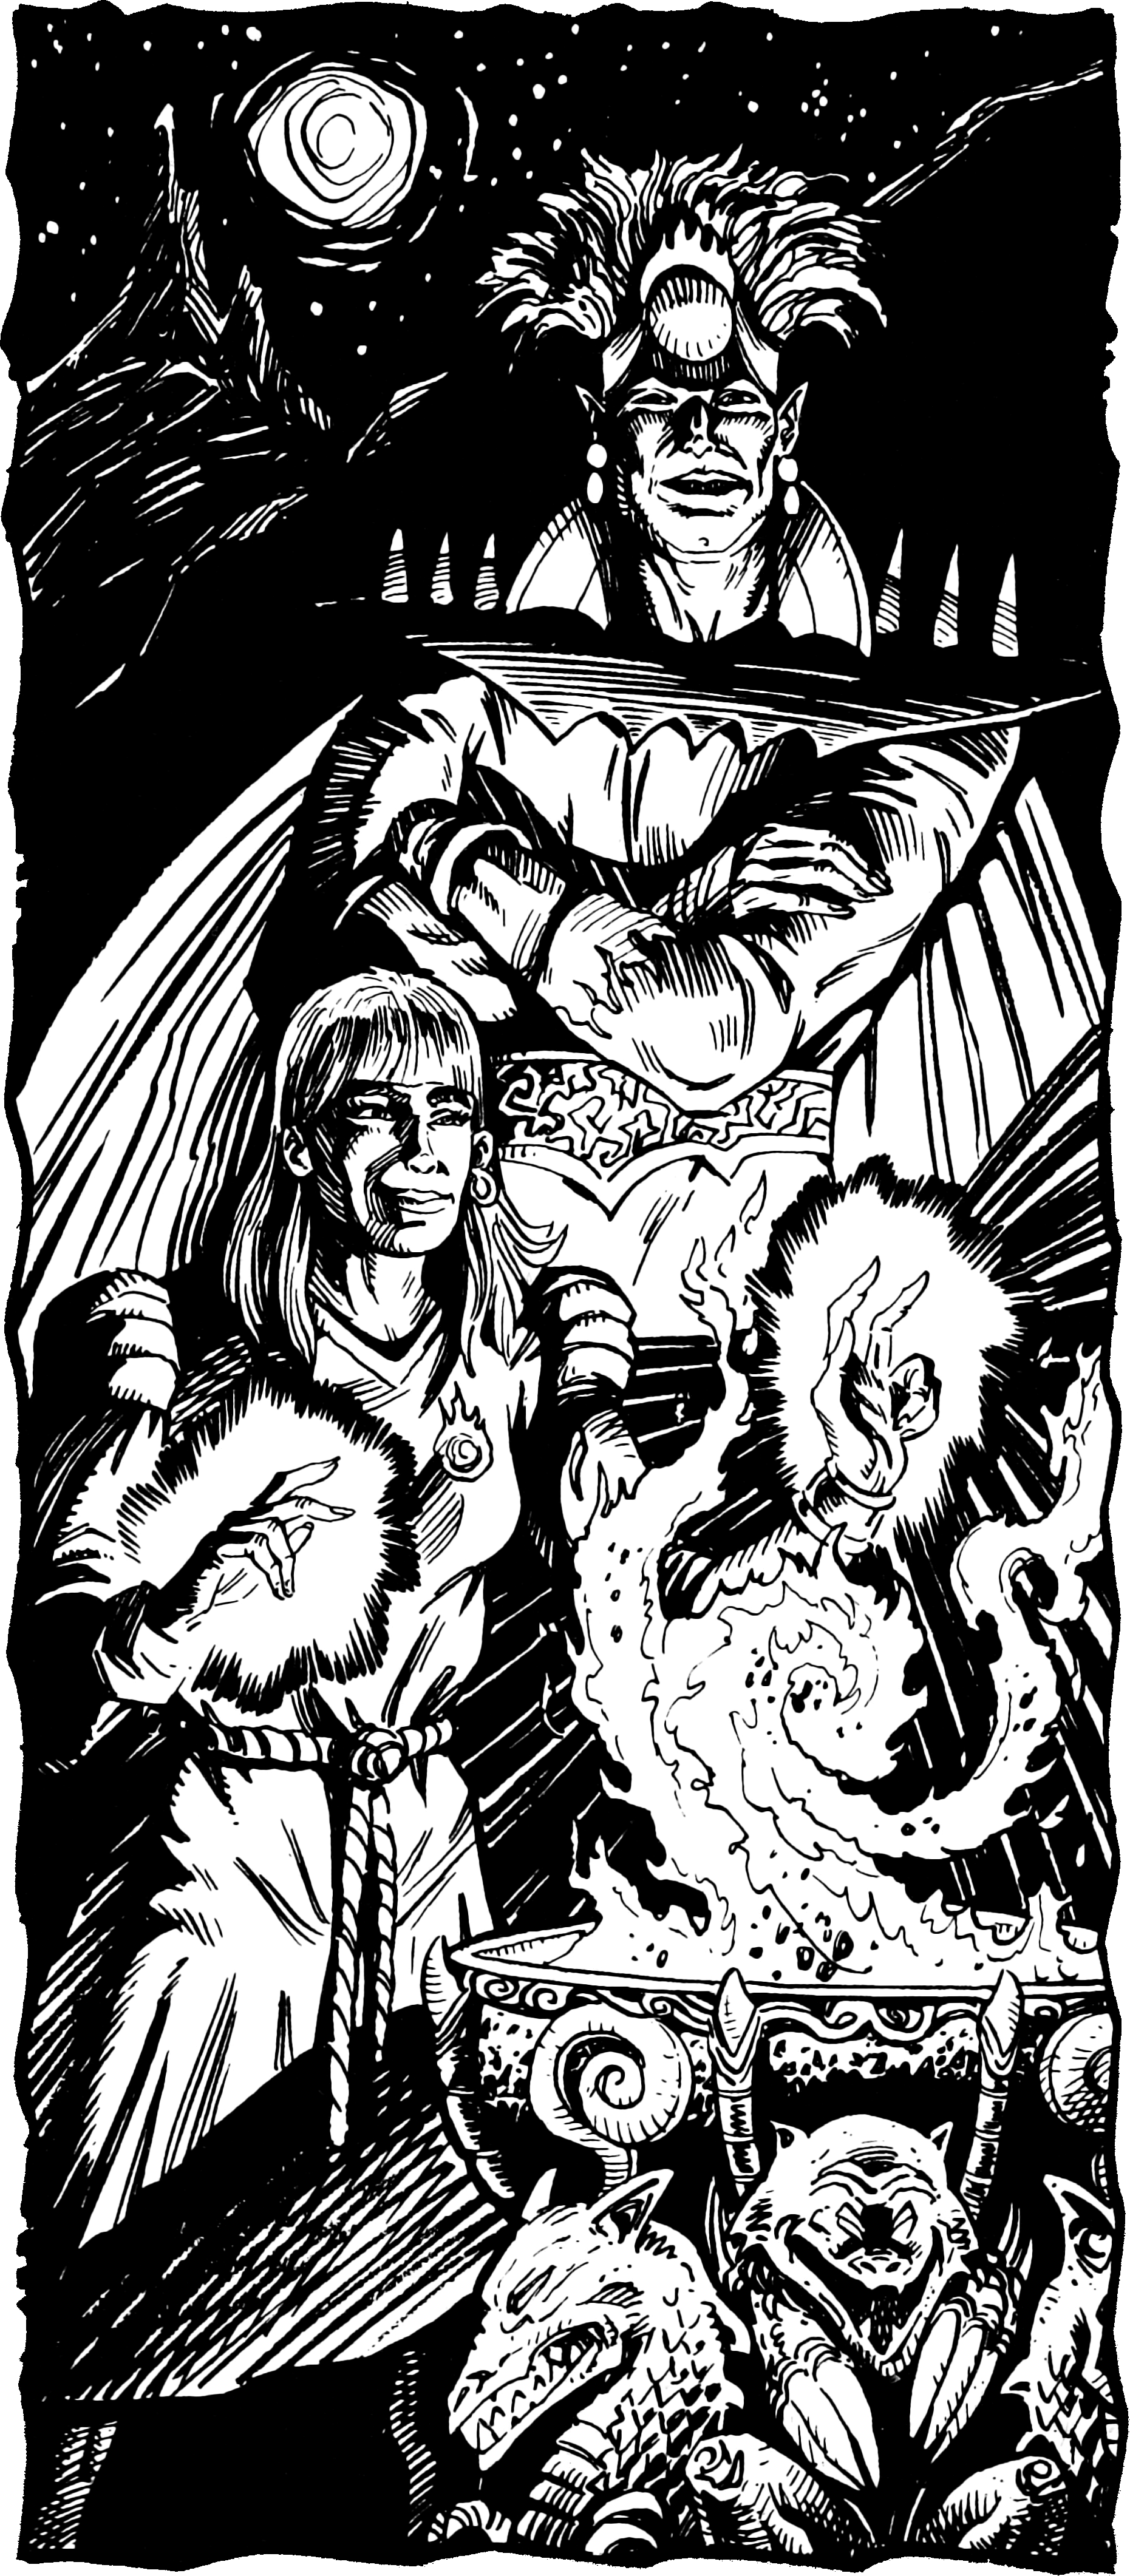
\includegraphics[width=\columnwidth+2mm]{images/cleric-2.png}
\par\textit{\small\textcopyright Wizards of the Coast, 2020.}
\end{figure}

\subsubsection{Friends \& Enemies}
Life under the crimison sun has no half measures. Your friends are tight, and your enemies are ruthless.

\begin{enumerate*}
\item Roll a die. On an even roll, they're male, otherwise they're female.
\item Roll a die. On an even roll, it's a friend---roll 1d10 and check the nature of the relationship on \tabref{Friend}. On an odd roll, it's an enemy---roll for each step in \tabref{Enemy}.
\end{enumerate*}

\Table{Friend}{lX}{
\textit{d10} & \tableheader Relationship\\
1 & Like a big sibling to you.\\
2 & Like a kid sibling to you.\\
3 & A teacher/mentor.\\
4 & A partner or co-worker.\\
5 & An old lover.\\
6 & An old enemy.\\
7 & Like a foster parent to you.\\
8 & A relative.\\
9 & Reconnect with an old childhood friend.\\
10 & Met through a common interest.\\
\rowcolor{white}\\
\rowcolor{white}\\
}

\begin{figure*}[b]
\centering
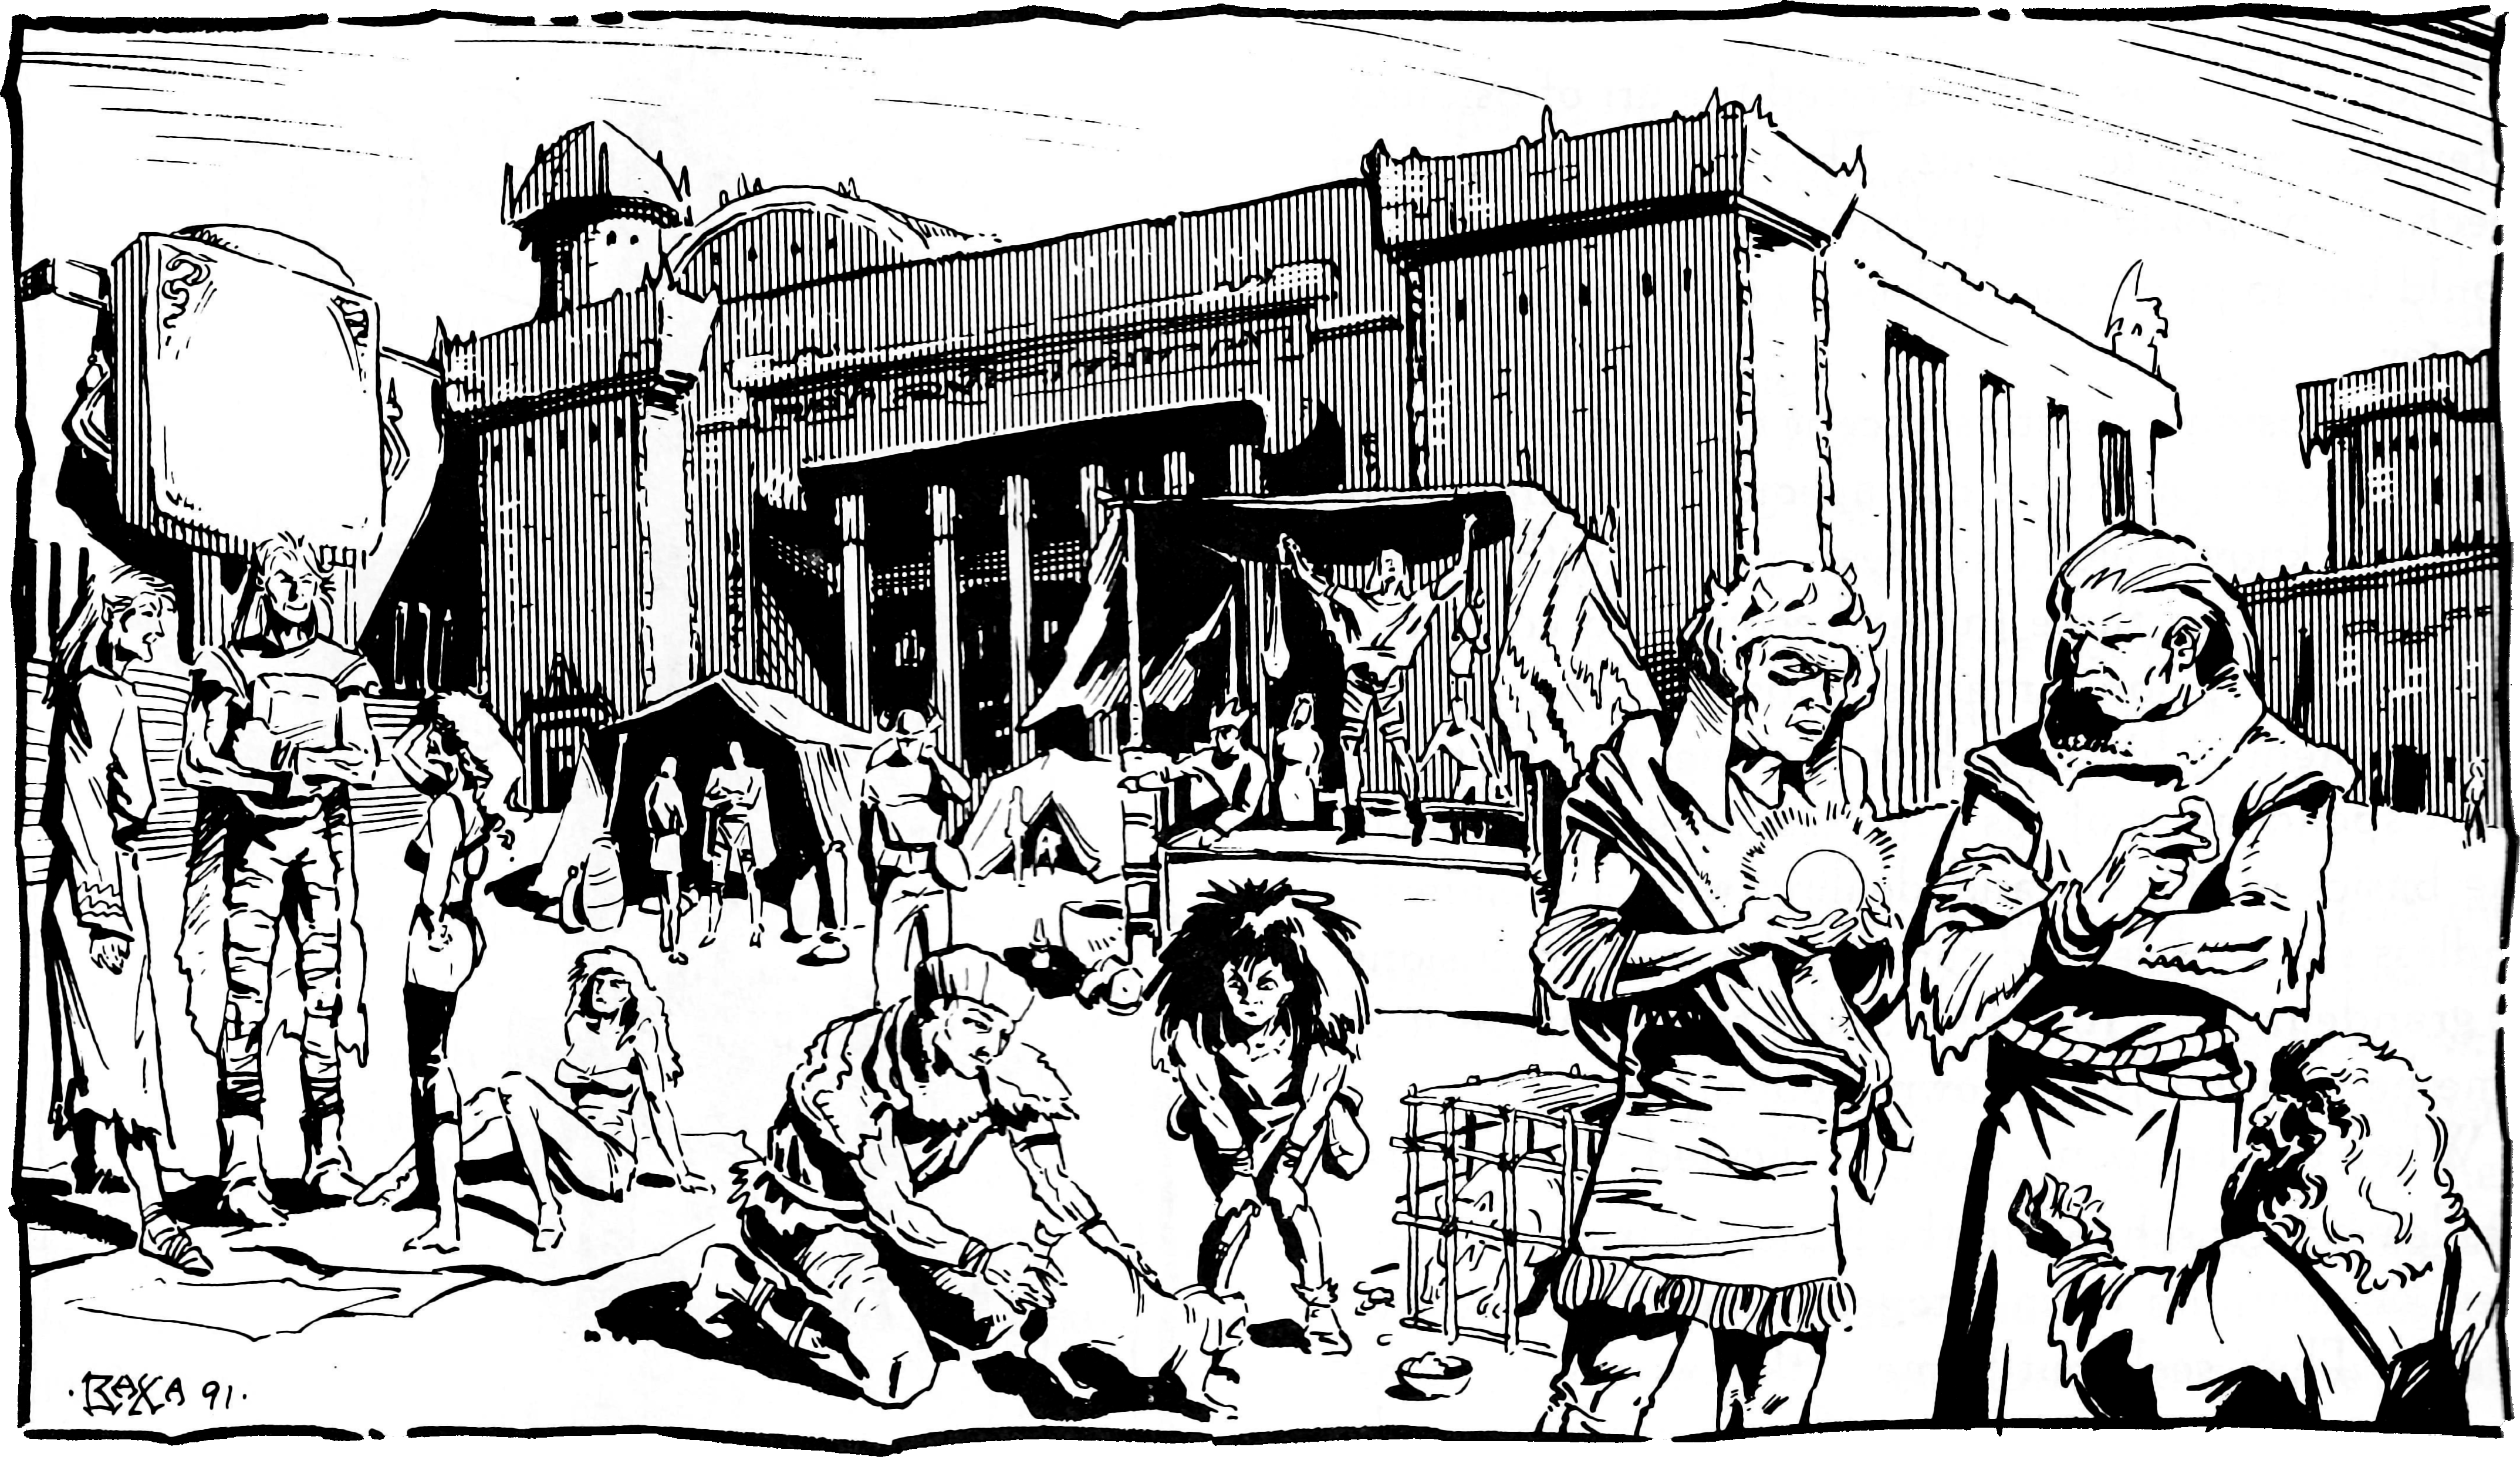
\includegraphics[scale=1.7]{images/market-1.png}
\par\textit{\small\textcopyright Wizards of the Coast, 2020.}
\end{figure*}
\Table{Enemy}{lX}{
\textit{d10} & \tableheader Who is your enemy... \\
1  & Ex-friend              \\
2  & Ex-lover               \\
3  & Relative               \\
4  & Childhood enemy        \\
5  & Person working for you \\
6  & Person you work for    \\
7  & Partner or co-worker   \\
8  & Veiled Alliance member \\
9  & Merchant House member  \\
10 & Templar                \\
% }
% \Table{Cause of Enmity}{lX}{
\rowcolor{white}\\
\textit{d10} & \tableheader Started wheh one of you... \\
1  & Caused the other to lose face or status.\\
2  & Caused the loss of a lover, friend or relative.\\
3  & Caused a major humiliation.\\
4  & Accused the other of cowardice or some other personal flaw.\\
5  & Caused a physical disability. Roll 1d6. 1--2: lost eye. 3--4: lost arm. 5--6: badly scarred.\\
6  & Deserted or betrayed the other.\\
7  & Turned down other's offer of job or romance.\\
8  & You just didn't like each other.\\
9  & Was a romantic rival.\\
10 & Foiled a plan of the other's.\\
% }
% \Table{Who is Mad at Who}{lX}{
\rowcolor{white}\\
\textit{d6} & \tableheader Who is mad? \\
1--2 & They hate you.\\
3--4 & You hate them.\\
5--6 & The feeling's mutual.\\
\cmidrule[0pt]{1-2}
% }
% \Table{Injured Party}{lX}{
\rowcolor{white}\\
\textit{d10} & \tableheader What the injured party will do? \\
1--2 & Go into murderous killing rage.\\
3--4 & Avoid the scum.\\
5--6 & Backstab them indirectly.\\
7--8 & Ignore the scum.\\
9--10 & Rip them verbally.\\
% }
% \Table{Enemy forces}{lX}{
\cmidrule[0pt]{1-2}
\rowcolor{white}\\
\textit{d10} & \tableheader What can your enemy use against you? \\
1--3 & Just themselves \\
4--5 & Themselves and a few friends \\
6--7 & An entire raider tribe \\
8 & A small merchant house \\
9 & A large merchant house \\
10 & The entire templarate \\
}

\subsubsection{Romance}

\Table{}{lX}{
\textit{d10}  &\tableheader How it worked out\\
1--4  & Happy love affair.\\
5--6  & Roll \tabref{Affair with Problems}.\\
7     & Roll \tabref{Tragic Love}.\\
8--10 & Fast affairs and hot dates.\\
}

\Table{Affair with Problems}{lX}{
\textit{d10} & \tableheader Problem\\
1 & Your lover's friends/family hate you.\\
2 & Your lover's friends/family would use any means to get rid of you.\\
3 & Your friends/family hate your lover.\\
4 & One of you has a romantic rival.\\
5 & You are separated in some way.\\
6 & You fight constantly.\\
7 & You're professional rivals.\\
8 & One of you is insanely jealous.\\
9 & One of you is ``messing around''.\\
10 & You have conflicting background and families.\\
}

\Table{Tragic Love}{lX}{
\textit{d10} & \tableheader What happened \\
1  & Lover died in accident.\\ 
2  & Lover mysteriously vanished.\\ 
3  & It didn't work out.\\ 
4  & A personal goal came between you.\\ 
5  & Lover kidnapped.\\ 
6  & Lover went insane.\\ 
7  & Lover commited suicide.\\ 
8  & Lover killed in a fight.\\ 
9  & Rival cut you out of the action.\\ 
10 & Lover imprisoned or exiled.\\ 

\rowcolor{white}\\
\textit{d10} & \tableheader Mutual feelings \\
1  & They still love you.\\
2  & You still love them.\\
3  & You still love each other.\\
4  & You hate them.\\
5  & They hate you.\\
6  & You hate each other.\\
7  & You're friends.\\
8  & No feelings either way; it's over.\\
9  & You like them, they hate you.\\
10 & They like you, you hate them.\\
}
